\chapter{Design} \label{chapter:design}
The design phase sets out to elaborate on the scenarios for experiments with IoT device. In these experiments, we compare and combine approaches from industry standards and papers presented in the analysis section. Conclusions are taken into consideration in establishing the plan of measurements and in the construction of the sensor unit.

\section{Research questions}
% Questions
% Goals
% Project risk management
This thesis aims to provide answers to four research questions. The focus is primarily on making data flow more efficient in an industrial sensor network that monitors rotating machines. The \textbf{research questions} are:
\begin{enumerate}[label=RQ\arabic*., font=\bfseries]
    \itemsep0pt
	\item Which temporal and spectral features can be extracted from vibration signals to provide the most accurate record of machinery faults?
	\item What is the reduction in transmission goodput when chosen signal features are used?
	\item What accuracy of prediction models can be achieved with various feature subsets?
	\item How can machinery faults be continuously identified and predicted based upon collected events?
\end{enumerate}

\noindent In accomplishing the objectives of our research we propose several \textbf{goals}:
\begin{todolist}
    \itemsep0pt
    \item Statistically and visually describe vibration signals from the Machinery fault database (MauFaulDa).
    \item Establish a list of conditions that should be later investigated in the experimental setting.
    \item Prepare dataset to be used in conjunction with machine learning models, namely by identifying labels and balancing classes.
    \item Find the best subsets of features in the temporal and spectral domain with previously analyzed feature extraction and selection methods.
    \item Evaluate the performance of models described in the diagnostics section with a significant focus on the k-nearest neighbor algorithm.
    \item Acquire measurements of vibrations from machines in the real environment to form a novel dataset of machinery behavior.
    \item Develop hardware and implement its firmware to obtain such measurements of the quality demanded by vibrodiagnostics standards.
\end{todolist}

However, we leave out from our efforts experiments on the data features calculated from wavelets and peaks in the spectral domain. The reason is that we did not find a way to represent extracted features more succinctly as a single number. We also did not discover a strategy for choosing only the relevant frequency bins. The assembled description is retained to lead further research on that topic.

The goals are impacted by certain \textbf{risks} that are assessed and tracked:

\begin{enumerate}[label=R-\arabic*., font=\bfseries]
\itemsep0pt
\item Machines in the real environment will not be available for vibration measurements. \\ \emph{Mitigation}: Contact and establish collaboration with alternative partners. 
\item Repeated measurements will not be consistent, and a lack of data is obtained from different classes.
\\ \emph{Mitigation}: Prepare a plan for measurements and photo document sensor placements. 
\item Fault modes can not be reliably differentiated and labeled in the dataset.
\\ \emph{Mitigation}: Consult domain experts and machine maintenance staff.
\item Suggestions made by exploring the MaFaulDa dataset will not be applicable in practice. \\
\emph{Mitigation}: When applicable, apply the same procedures as in MaFaulDa to measured data.
\end{enumerate}


\section{Machine learning pipeline}
% UML pipeline (fig.) and parameters

Dataset scenarios - 24 scenarios
\begin{itemize}
\item domain - TD, FD
\item dim - 1, 3
\item bearing - A, B, A+B
\item severity - No, Yes
\end{itemize}

\begin{figure}[h]
    \centering
	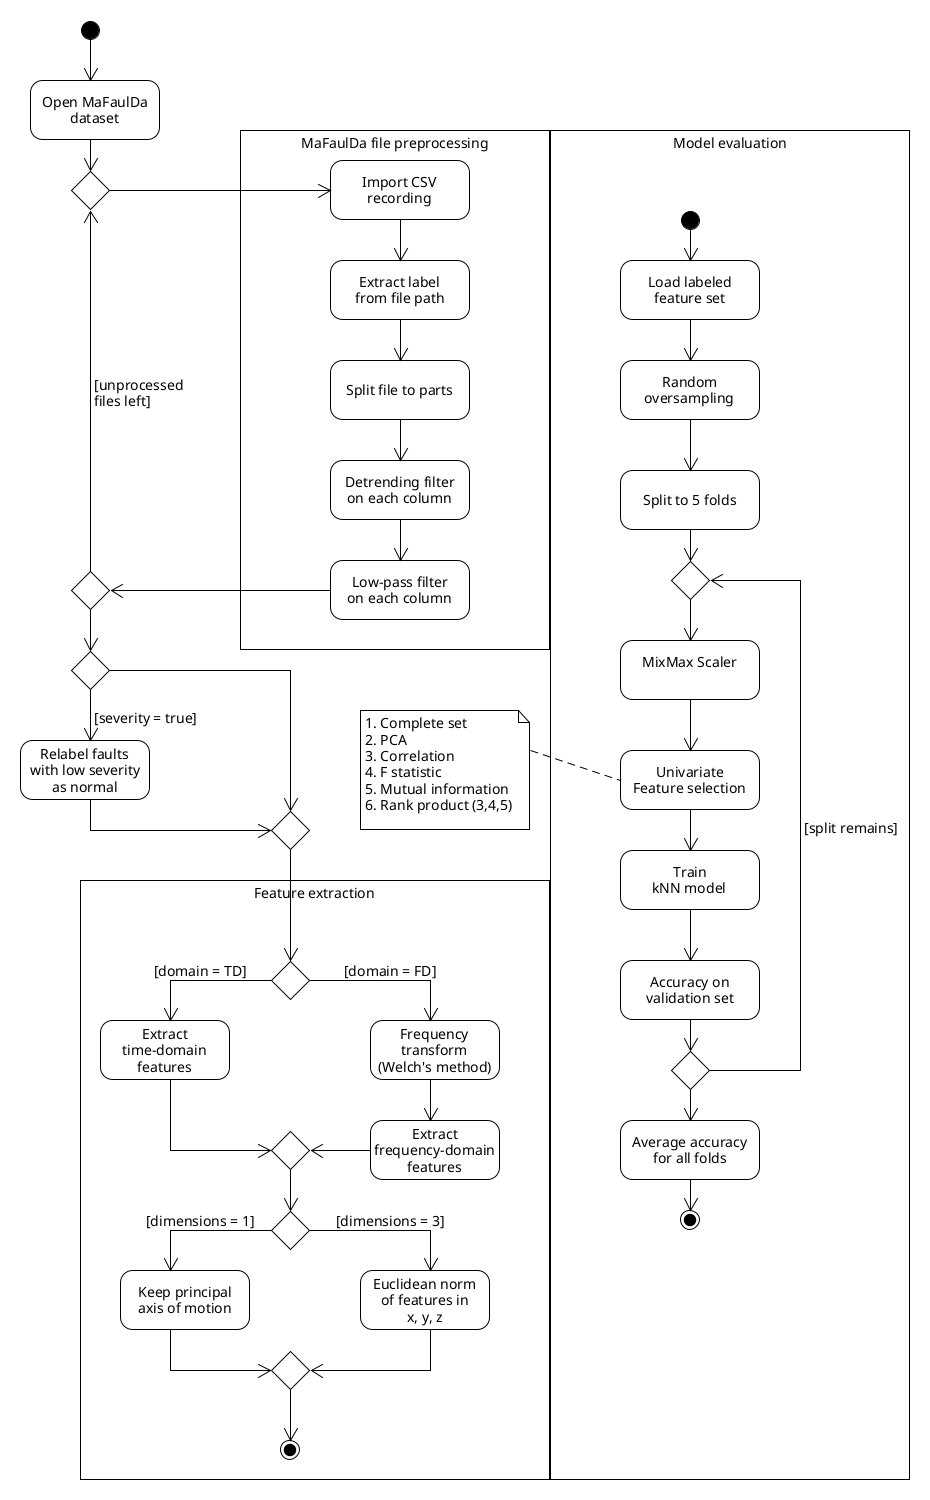
\includegraphics[width=\textwidth]{assets/design/pipeline-design.png}
\end{figure} 


% Experiments and metrics:
\begin{itemize}
\item Complete feature sets
\item Feature combinations
\item Feature selection methods
\item Incremental learning
\item Clustering - Silouette score
\end{itemize}


\section{Exploratory data analysis of MaFaulDa}
% Fault counts
\begin{table}[h]
\centering
\begin{tabular}{|l|l|l|l|l|l|l|l|l|}
\hline
\textbf{Bearings} & \textbf{Severity} & \textbf{Misalignment} & \textbf{Imbalance} & \textbf{Cage fault} & \textbf{Ball fault} & \textbf{Outer race fault} & \textbf{Normal} & \textbf{$\Sigma$} \\ \hline
A                 & No                & 498                   & 333                & 188                 & 186                 & 184                       & 49              & 1438              \\ \hline
B                 & No                & 498                   & 333                & 188                 & 137                 & 188                       & 49              & 1393              \\ \hline
A+B               & No                & 996                   & 666                & 376                 & 323                 & 372                       & 98              & 2831              \\ \hline
A                 & Yes               & 248                   & 188                & 91                  & 87                  & 86                        & 738             & 1438              \\ \hline
B                 & Yes               & 248                   & 188                & 90                  & 45                  & 90                        & 732             & 1393              \\ \hline
A+B               & Yes               & 496                   & 376                & 181                 & 132                 & 176                       & 1470            & 2831              \\ \hline
\end{tabular}
\end{table}

% Correlation to RPM
\begin{figure}[h]
    \centering
    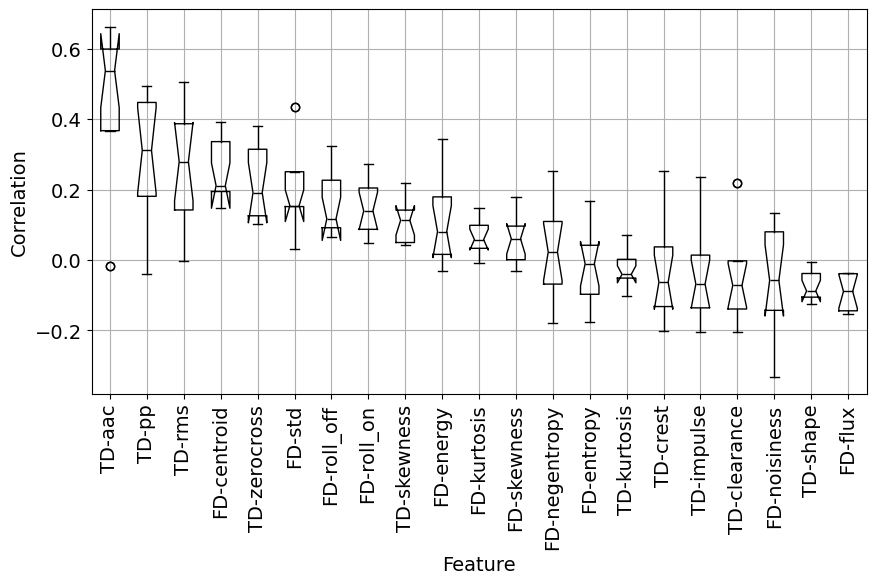
\includegraphics[width=0.5\textwidth]{assets/results/feature-values/corr-to-rpm.png}
    \caption{Correlation of features to RPM over all experiments}
\end{figure}


% Features Range
% Mafaulda
\begin{figure}[h]
    \centering
    \begin{subfigure}[b]{0.48\textwidth}
        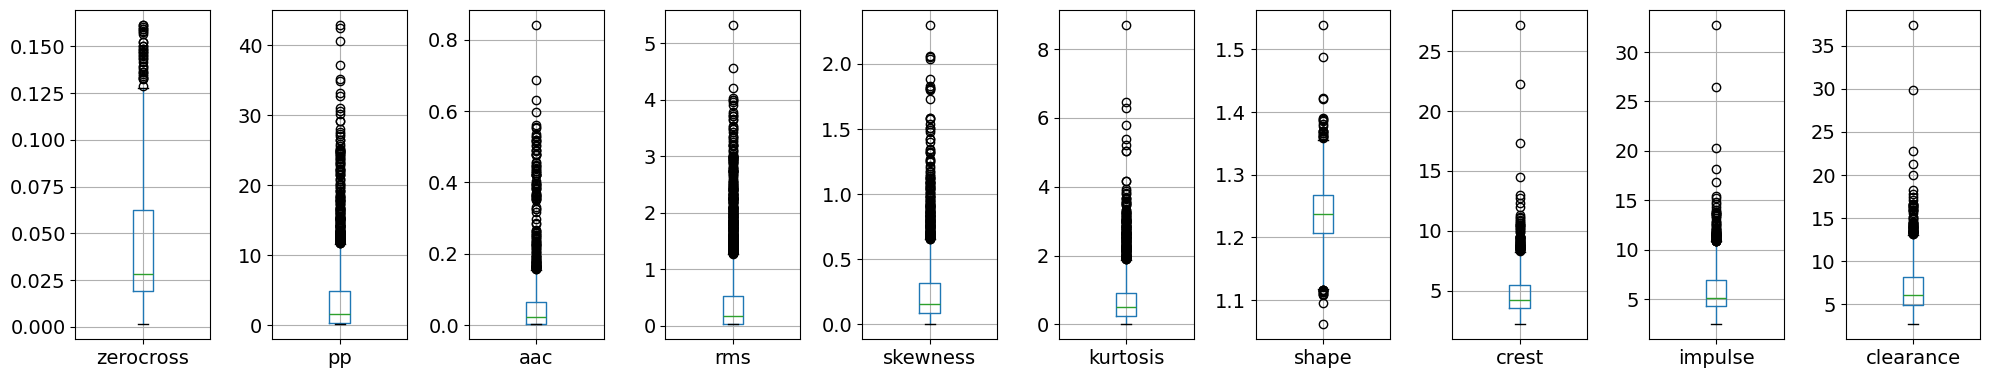
\includegraphics[width=\textwidth]{assets/results/feature-values/features-TD-dim1-A+B.png}
        \caption{Time-domain features}
    \end{subfigure}
    \hfill
    \begin{subfigure}[b]{0.48\textwidth}
        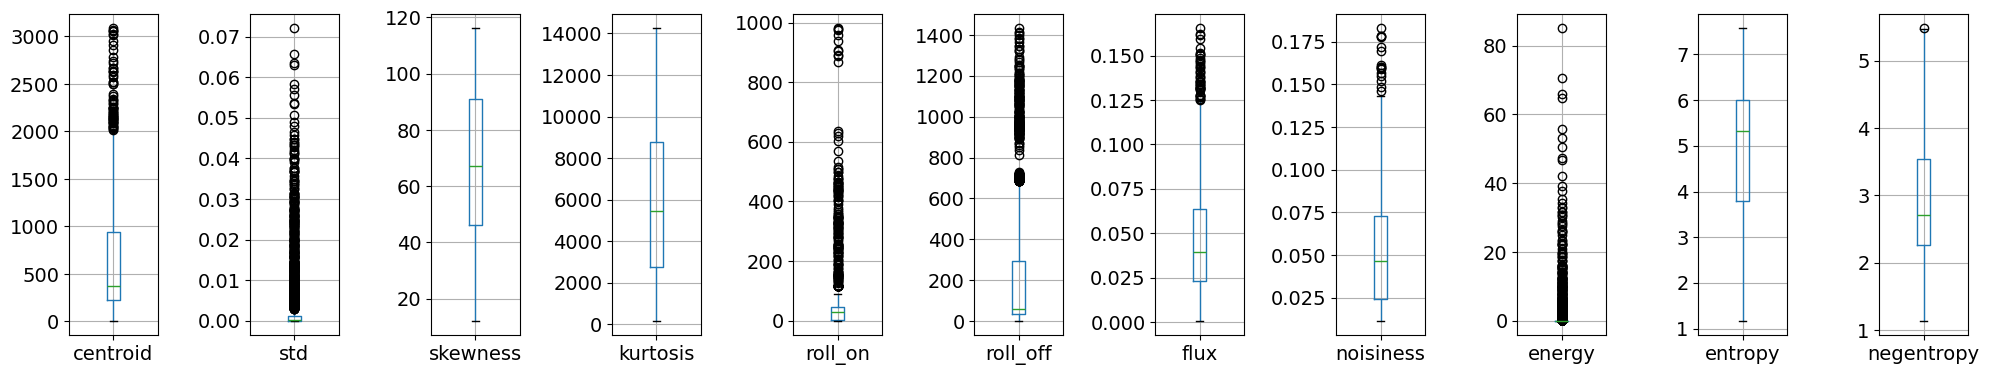
\includegraphics[width=\textwidth]{assets/results/feature-values/features-FD-dim1-A+B.png}
        \caption{Frequency-domain features}
    \end{subfigure}
    \begin{subfigure}[b]{0.48\textwidth}
        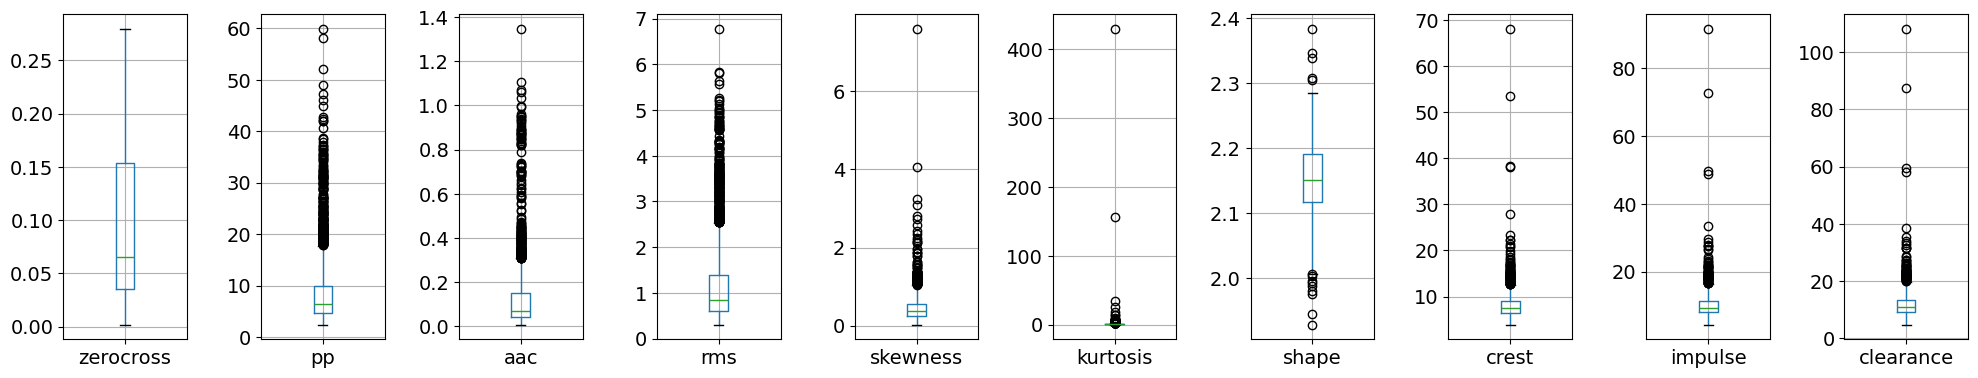
\includegraphics[width=\textwidth]{assets/results/feature-values/features-TD-dim3-A+B.png}
        \caption{Time-domain features}
    \end{subfigure}
    \hfill
    \begin{subfigure}[b]{0.48\textwidth}
        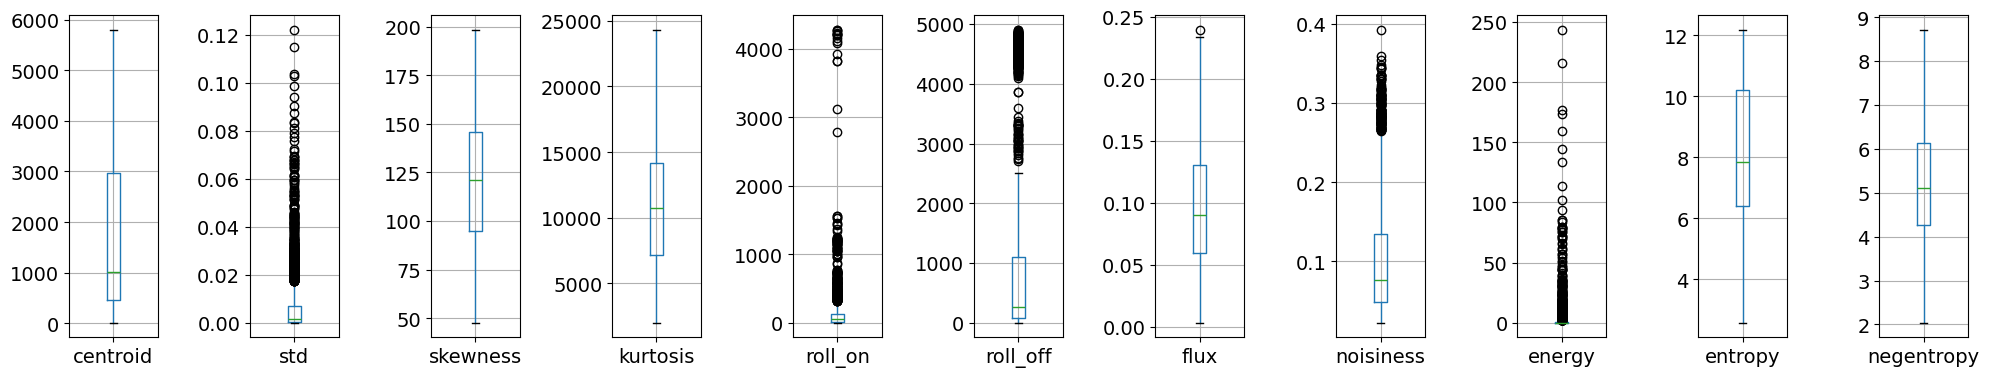
\includegraphics[width=\textwidth]{assets/results/feature-values/features-FD-dim3-A+B.png}
        \caption{Frequency-domain features}
    \end{subfigure}
    \caption{Feature range in MaFaulDa}
\end{figure}

% PCA plot of labels
% Clusters with true labels
\begin{figure}[h]
    \centering
    \begin{subfigure}[b]{0.48\textwidth}
        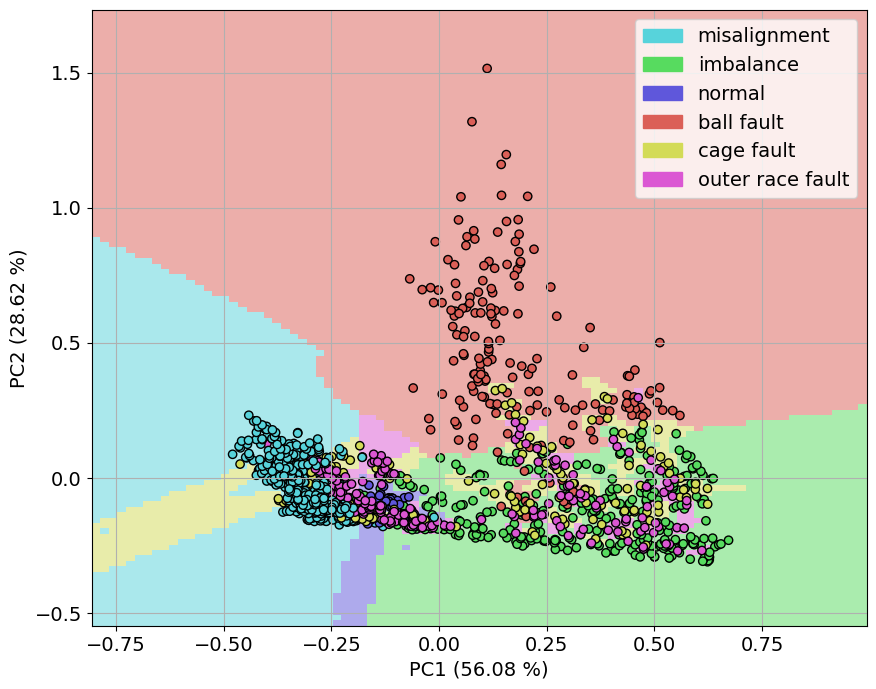
\includegraphics[width=\textwidth]{assets/results/labels/PCA-TD.png}
        \caption{Time-domain features}
    \end{subfigure}
    \hfill
    \begin{subfigure}[b]{0.48\textwidth}
        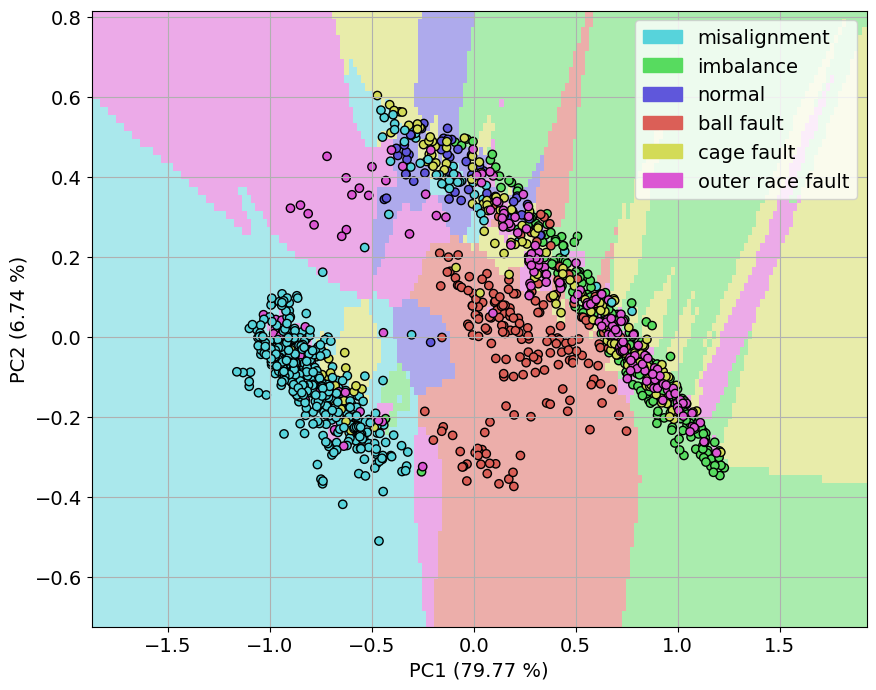
\includegraphics[width=\textwidth]{assets/results/labels/PCA-FD.png}
        \caption{Frequency-domain features}
    \end{subfigure}
    \hfill
    \begin{subfigure}[b]{0.48\textwidth}
        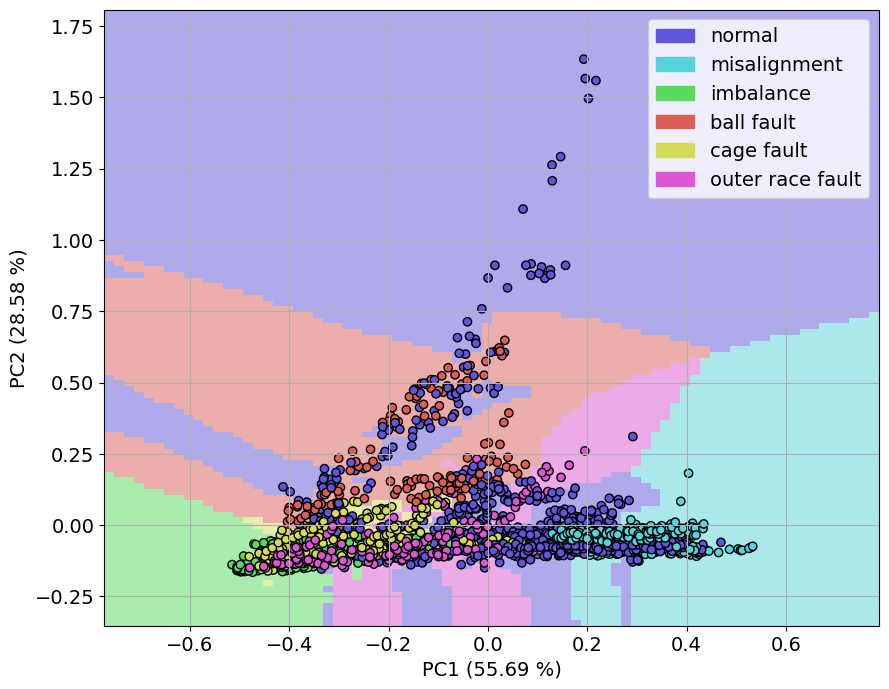
\includegraphics[width=\textwidth]{assets/results/labels/PCA-TD-severity.png}
        \caption{Time-domain features (severity)}
    \end{subfigure}
    \hfill
    \begin{subfigure}[b]{0.48\textwidth}
        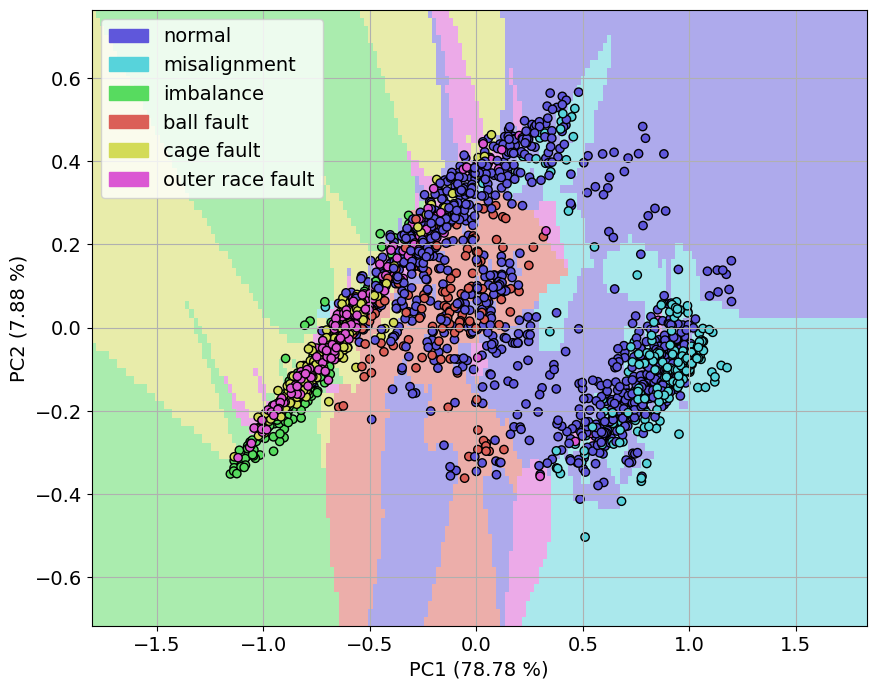
\includegraphics[width=\textwidth]{assets/results/labels/PCA-FD-severity.png}
        \caption{Frequency-domain features (severity)}
    \end{subfigure} 
    \caption{PCA of all features to 2 components}
\end{figure}

% Time domain waveforms of different faults
\begin{figure}[h]
    \centering
    \begin{subfigure}[b]{0.49\textwidth}
        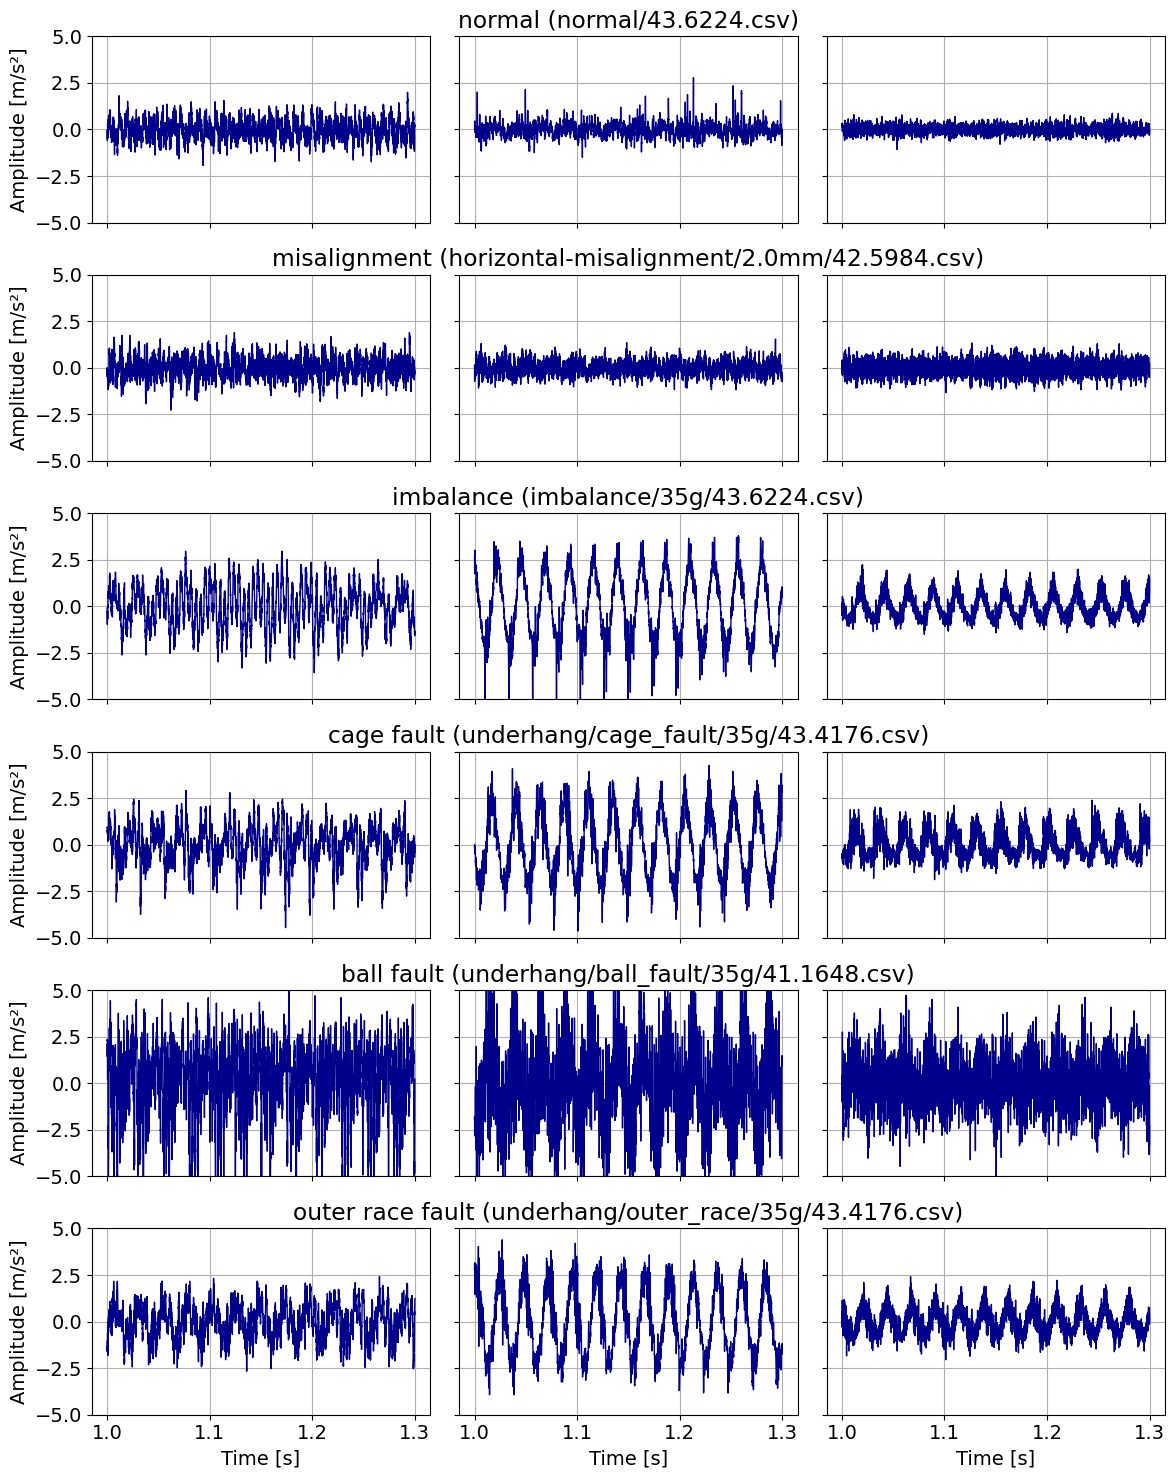
\includegraphics[width=\textwidth]{assets/results/eda/mafaulda-TD-A.png}
        \caption{Time domain}
    \end{subfigure}
    \hfill
    \begin{subfigure}[b]{0.49\textwidth}
        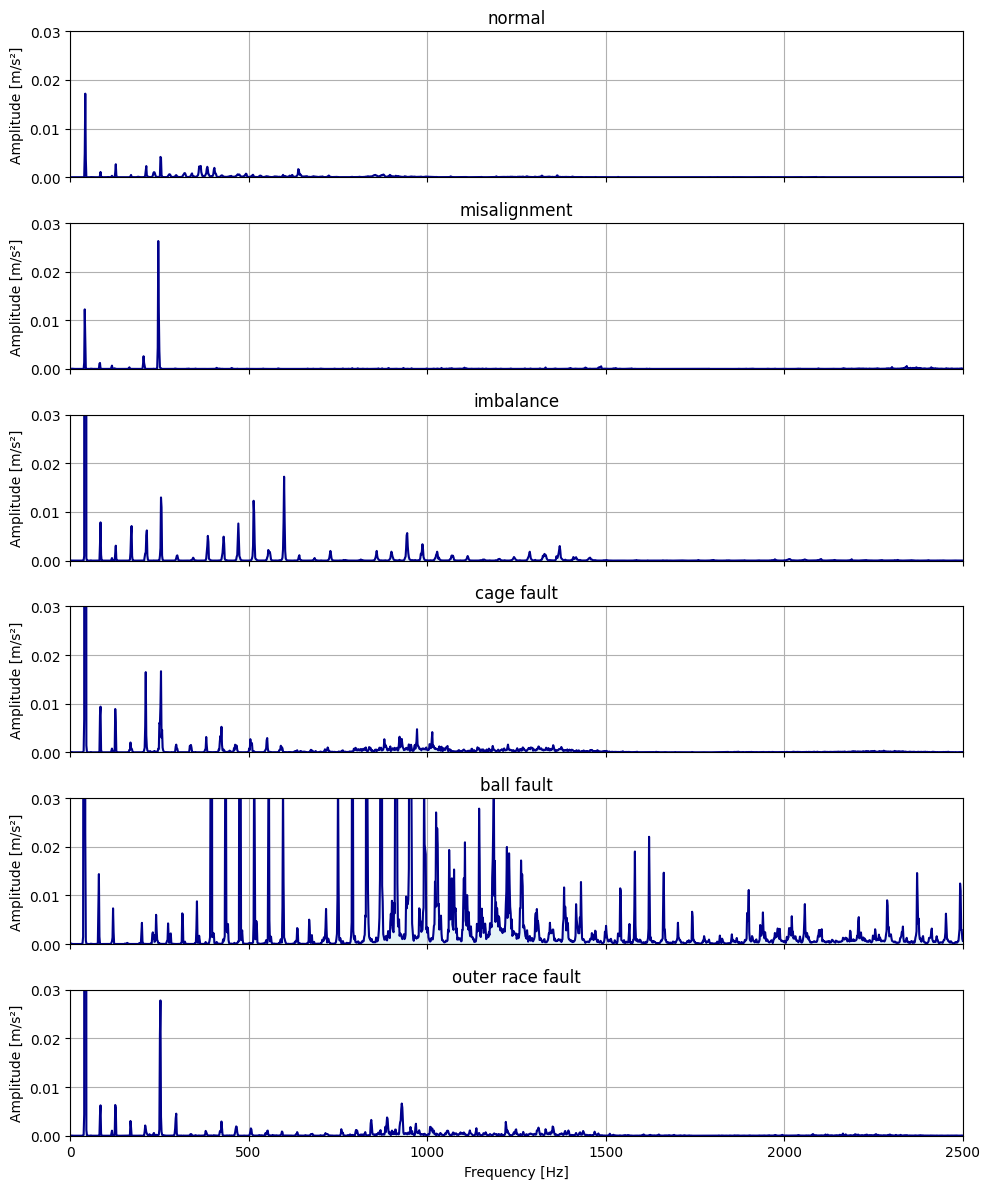
\includegraphics[width=\textwidth]{assets/results/eda/mafaulda-faults.png}
        \caption{Frequency domain (around 2500 rpm)}
    \end{subfigure}
    \caption{MaFaulDa}
\end{figure}


% PCA loading plots
\begin{figure}[h]
    \centering
    \begin{subfigure}[b]{\textwidth}
        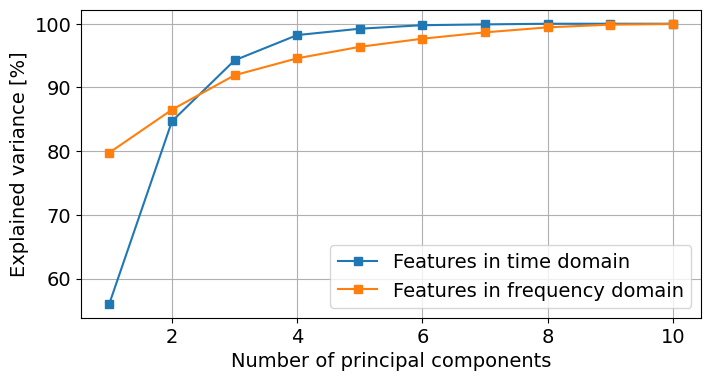
\includegraphics[width=\textwidth]{assets/results/eda/PCA-explained-variance.png}
        \caption{Time-domain features}
    \end{subfigure}
    \hfill
    \begin{subfigure}[b]{0.48\textwidth}
        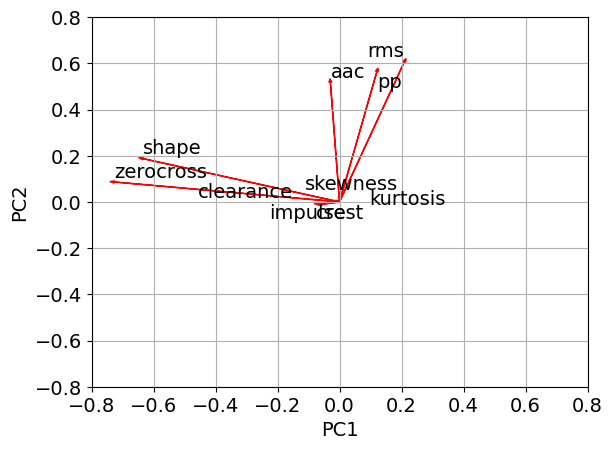
\includegraphics[width=\textwidth]{assets/results/eda/PCA-TD-loading-plot.png}
        \caption{Frequency-domain features}
    \end{subfigure}
    \hfill
    \begin{subfigure}[b]{0.48\textwidth}
        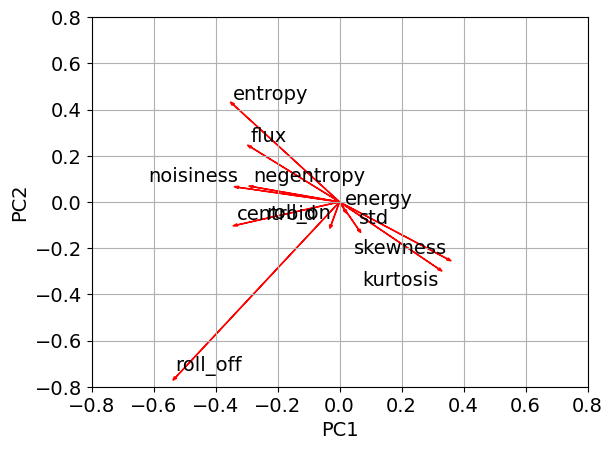
\includegraphics[width=\textwidth]{assets/results/eda/PCA-FD-loading-plot.png}
        \caption{Time-domain features (severity)}
    \end{subfigure} 
    \caption{PCA explained variance and loading plots (A bearing)}
\end{figure}



\section{Accelerometer data logger}
% Block diagram of device

% HW parameters and mention temporary device
\begin{table}[ht]
\renewcommand{\arraystretch}{1.2}
\centering
\begin{tabular}{|l|l|l|}
\hline
\textbf{Accelerometer}                           & \textbf{IIS3DWB}   \\ \hline
\textbf{Vendor}                                  & STMicroelectronics \\ \hline
\textbf{Bus}                                     & SPI                \\ \hline
\textbf{Axis}                                    & 1 or 3             \\ \hline
\textbf{Range} (g)                               & $\pm$ 2 - 16      \\ \hline
\textbf{Bandwidth} (kHz)                          & 5 - 6.3            \\ \hline
\textbf{Sensitivity} (mg/LSB)                    & 0.06 - 0.49       \\ \hline
\textbf{Noise density} ($\mu g / \sqrt{\mathrm{Hz}}$ rms) & 75                 \\ \hline
\textbf{Microcontroller}                         & ESP32-PoE-ISO      \\ \hline
\textbf{CPU SoC}                                 & ESP32-WROOM-32     \\ \hline
\textbf{Output data rate} (kHz)                  & 26.7               \\ \hline
\textbf{ADC resolution} (bit)                    & 16                 \\ \hline
\textbf{FIFO}                                    & 3 kB (512 samples) \\ \hline
\end{tabular}
\caption{Hardware parameters of previous and proposed sensor units}
\label{tab:design:hw-sensors}
\end{table}

\begin{figure}[h]
	\centering
	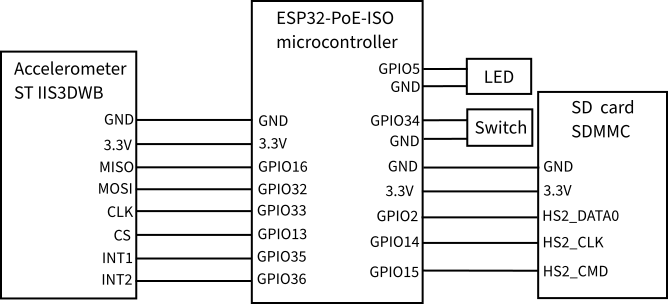
\includegraphics[width=0.9\textwidth]{assets/design/hw-block-schematic.png}
	\caption{Sensor unit hardware block diagram}
	\label{fig:design:block-diagram-hw}
\end{figure}

% Task communication sequence diagram

% Firmware
% Timing is crutial 19ms.
Activity diagrams describe three basic actions of firmware for logging accelerometer samples:

\begin{itemize}
\itemsep0pt
\item begin new recording, 
\item log block of samples into CSV file,
\item finish recording.
\end{itemize}

\begin{figure}[h]
    \centering
	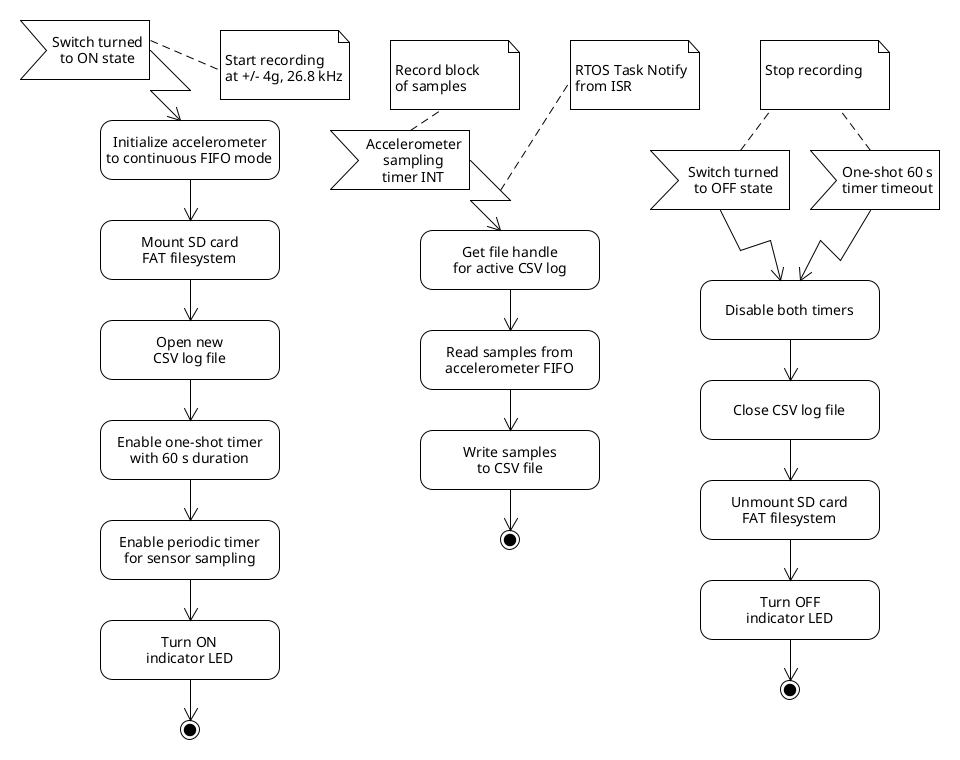
\includegraphics[width=\textwidth]{assets/design/firmware-design.png}
\end{figure} 


\section{Industrial equipment}
Three kinds of rotating machines are at disposal for vibration measurements. Those are a standing fan, scroll compressor, and water pump.

\begin{figure}[ht]
    \centering
    \begin{subfigure}[b]{0.17\textwidth}
    		\centering
        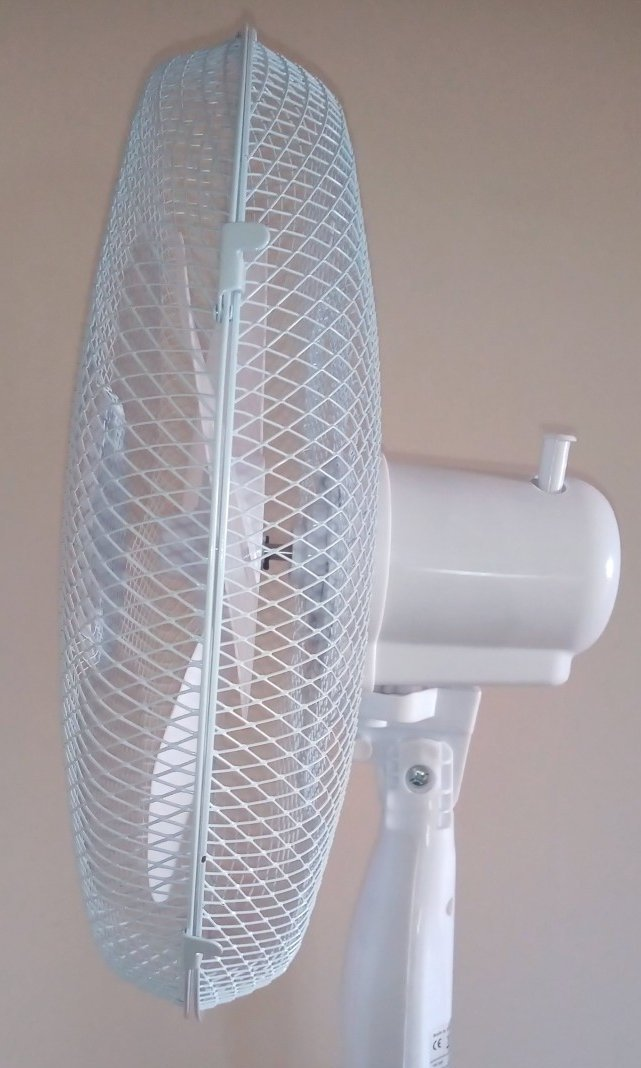
\includegraphics[width=\textwidth]{assets/design/machine-fan.jpg}
        \caption{\footnotesize Fan}
        \label{fig:machine:fan}
    \end{subfigure}
    \hfill
    \begin{subfigure}[b]{0.25\textwidth}
    		\centering
        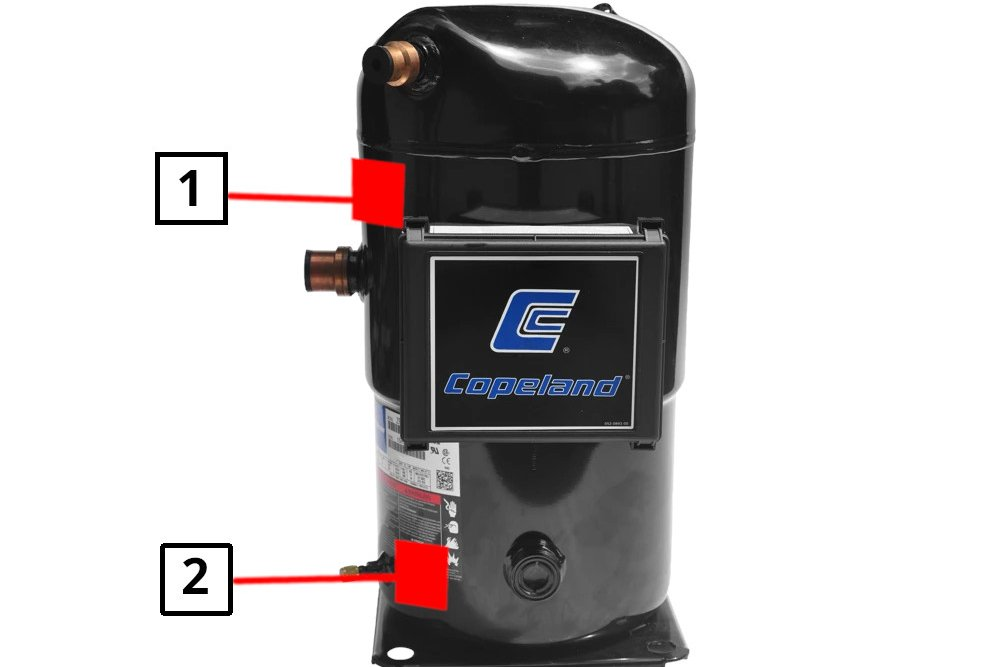
\includegraphics[width=\textwidth]{assets/design/sensor/copeland-compressor.jpg}
        \caption{\footnotesize Compressor}
        \label{fig:machine:compressor}
    \end{subfigure}
    \hfill
    \begin{subfigure}[b]{0.31\textwidth}
    		\centering
        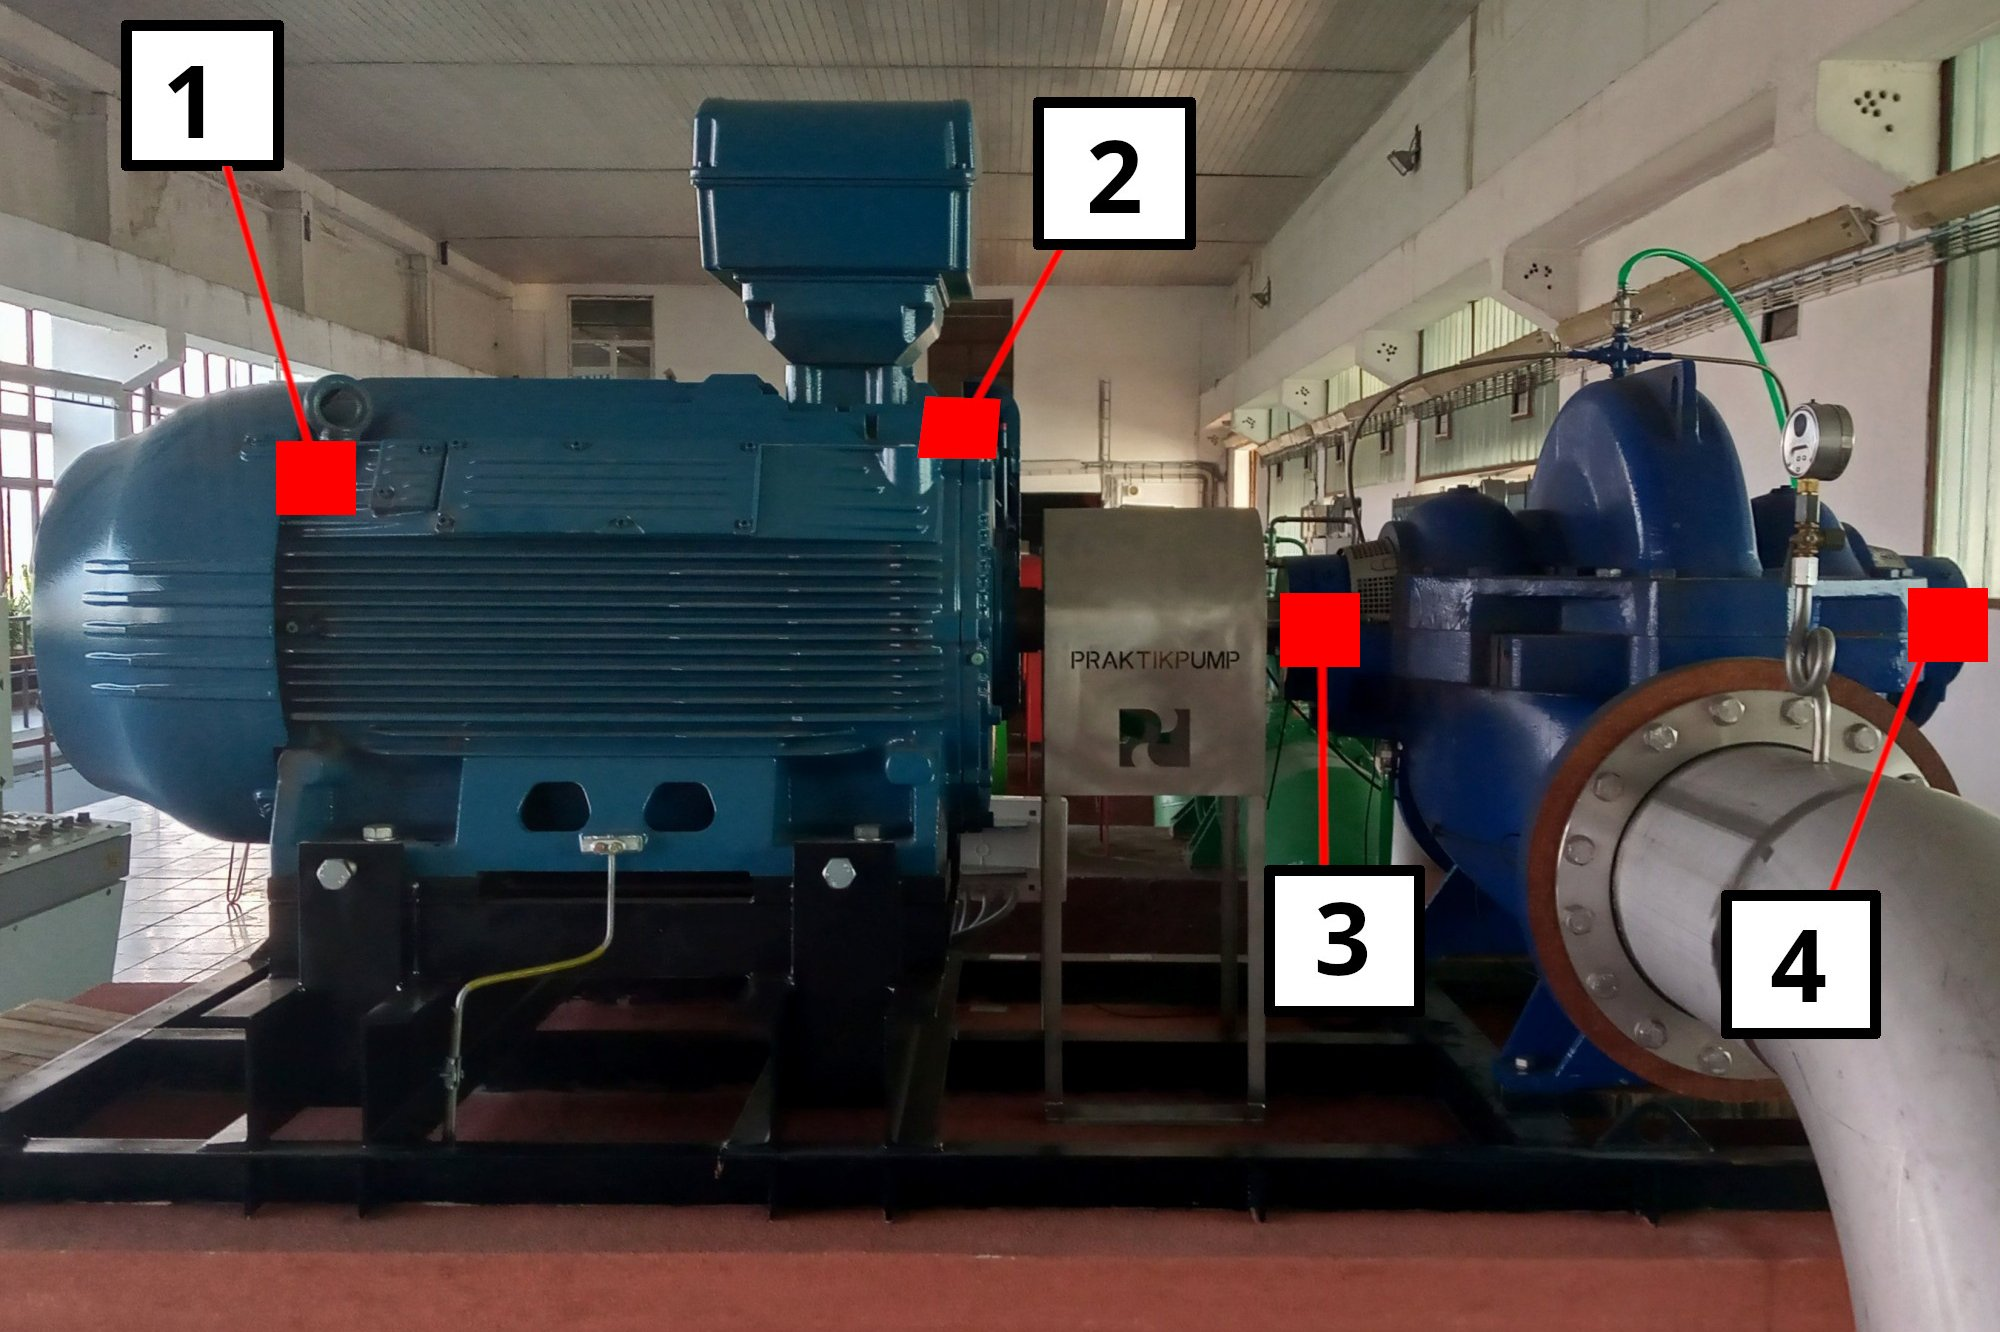
\includegraphics[width=\textwidth]{assets/design/sensor/ksb-pump.jpg}
        \caption{\footnotesize Water pump KSB}
        \label{fig:machine:pump-ksb}
    \end{subfigure}
    \hfill
    \begin{subfigure}[b]{0.31\textwidth}
    		\centering
        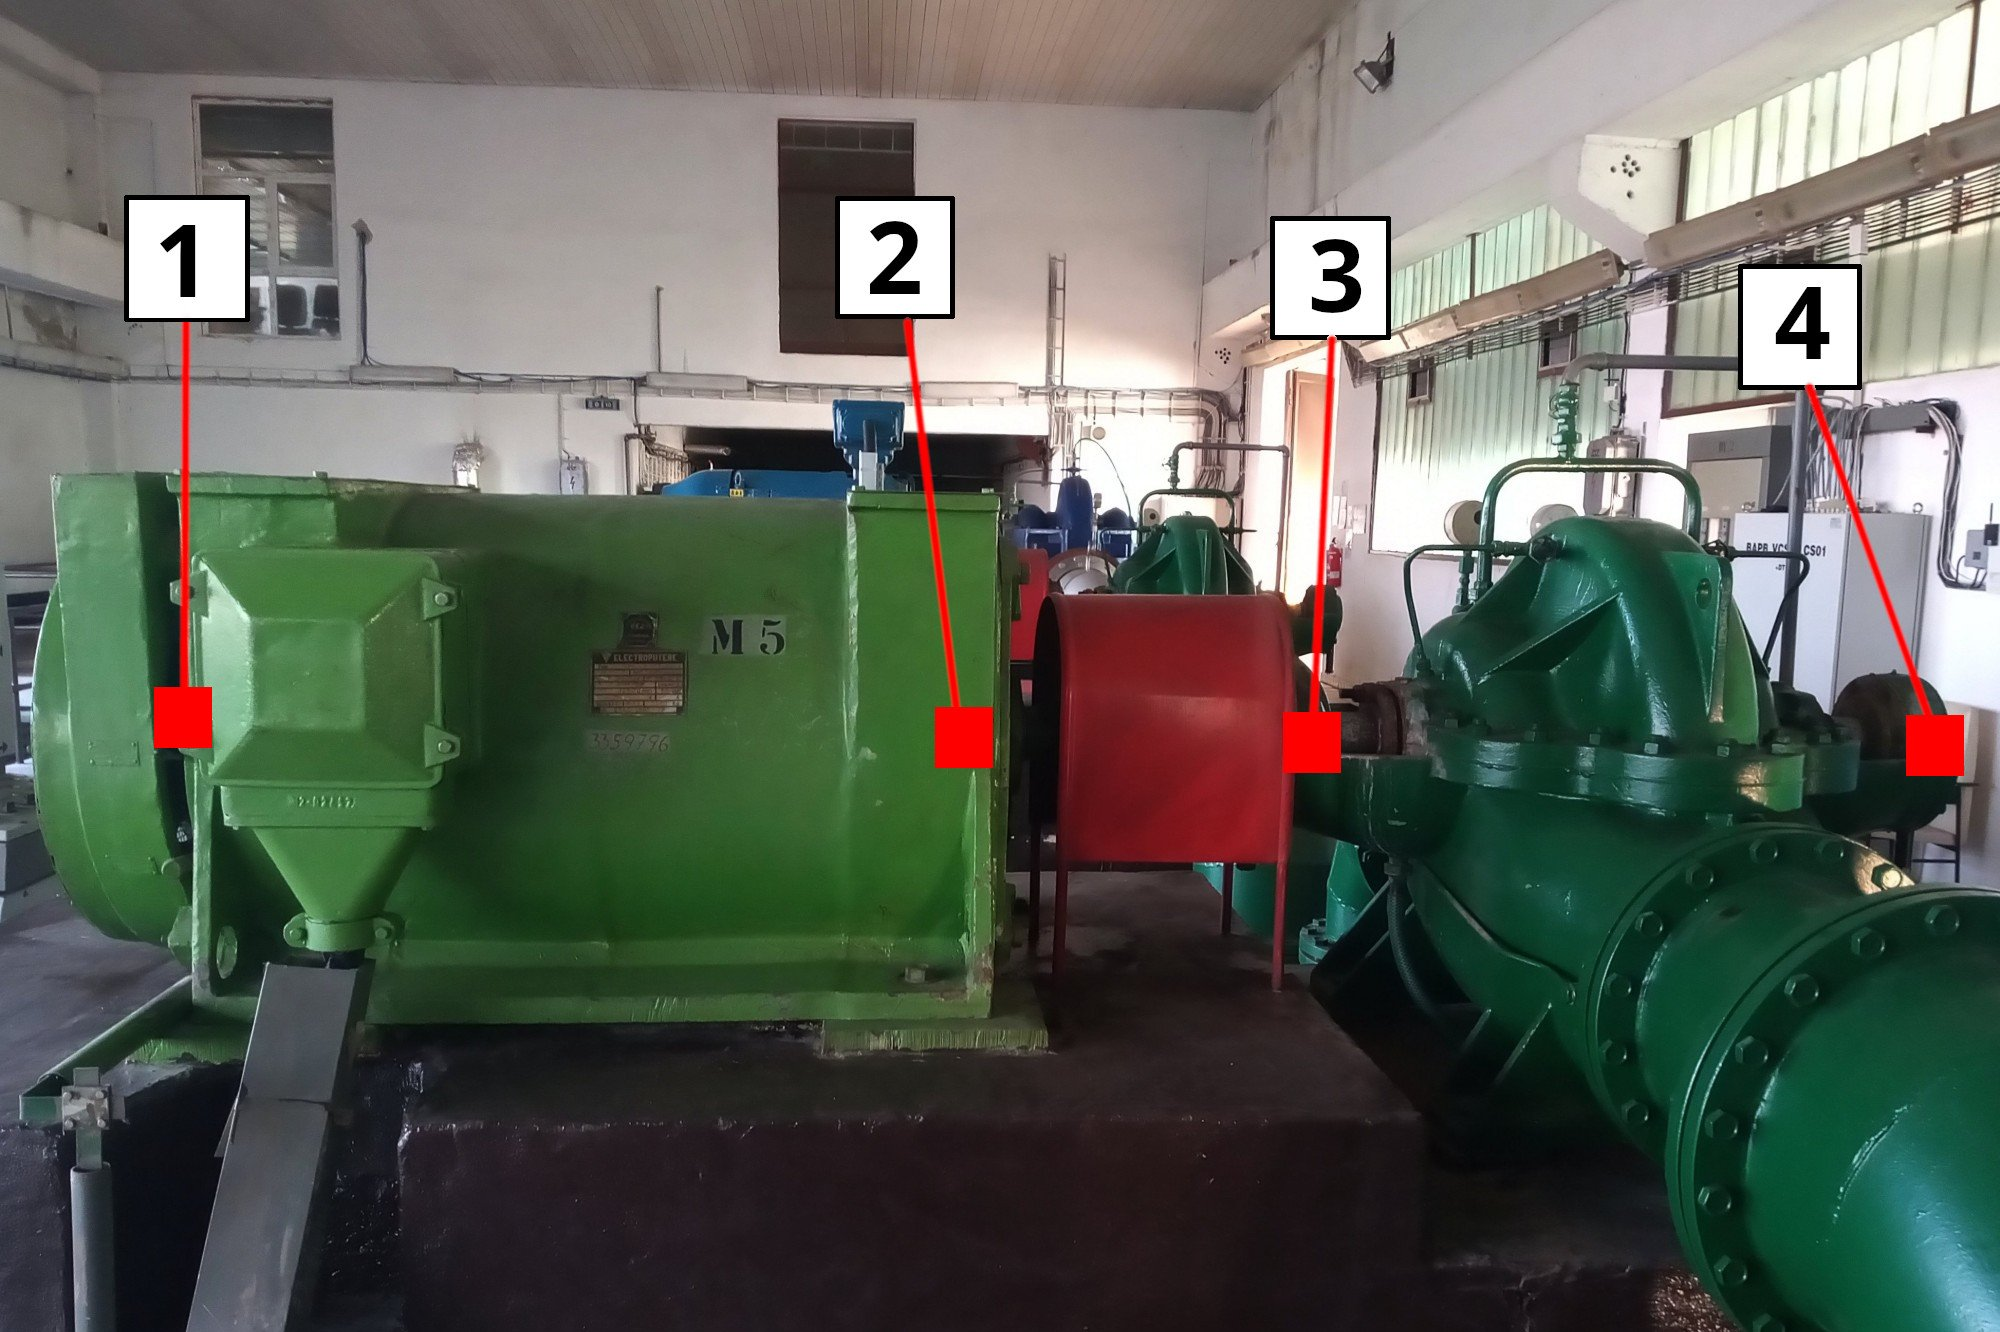
\includegraphics[width=\textwidth]{assets/design/sensor/sigma-pump.jpg}
        \caption{\footnotesize Water pump Sigma}
        \label{fig:machine:pump-sigma}
    \end{subfigure}
    \caption{Machines dedicated for vibration measurements}
\end{figure}

\textbf{Standing fan} is model \emph{Kalorik~TKG~VT1037} (Fig.~\ref{fig:machine:fan}) and one unit is available to us. It serves as a test bed during the sensor unit development. The sensor is placed on the plastic casing at the back of the drive motor. The fan has a 45~cm diameter with 3~propellers and a power of 45~W (class~\rom{1}). It has a switch for 3 rotational speeds, which are approximately 18.5~Hz (1100~rpm), 20.4~Hz (1200~rpm), and 22~Hz (1300~rpm).

\textbf{Scroll compressor} is model \emph{Copeland~ZR16} (Fig.~\ref{fig:machine:compressor}). Altogether, two units are available in two independent air conditioning units for the data center. The compressor has 9.7~kW of power (class~\rom{1}) and rotates at 2900 rpm (48.3 Hz). Two possible measurement locations are located on the sides on top of the bearings, just above the base and above the scroll.

\textbf{Water pumps} are available as 3 units in municipal drinking water pumping station. The apparatus consists of a single-stage axially split volute casing pump and an attached electric induction motor. 

The newer primary pumps with bundled wireless cloud monitoring system are two units of \emph{KSB Omega~300-560} (Fig.~\ref{fig:machine:pump-ksb}). The pumps were commissioned in 2018, and they rotate at 1493 rpm (24.9 Hz). The electric motor provides 400~kW of power (class~\rom{3}).

The secondary pump is one unit named \emph{Sigma~300-OVD-600} (Fig.~\ref{fig:machine:pump-sigma}) installed in 1986. It rotates at 1485 rpm (24.75 Hz), and its electric motor has power of 450~kW (class~\rom{3}). Each pump and motor have 2 bearings. Therefore, there are 4 measurement positions in total.

\begin{figure}[h]
    \centering
    \begin{subfigure}[b]{0.49\textwidth}
    		\centering
        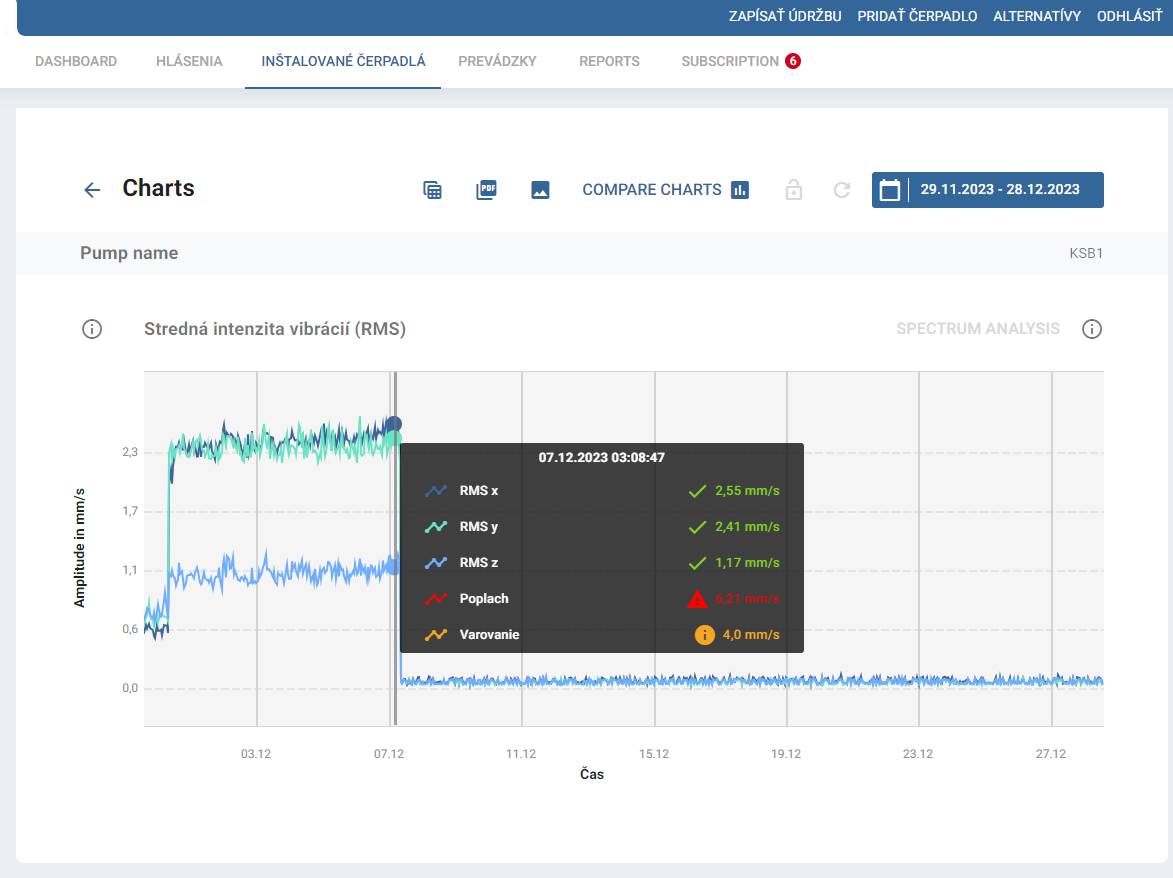
\includegraphics[width=\textwidth]{assets/design/ksb-guard-rms.png}
        \caption{Vibration rms velocity dashboard}
    \end{subfigure}
    \hfill
    \begin{subfigure}[b]{0.49\textwidth}
    		\centering
        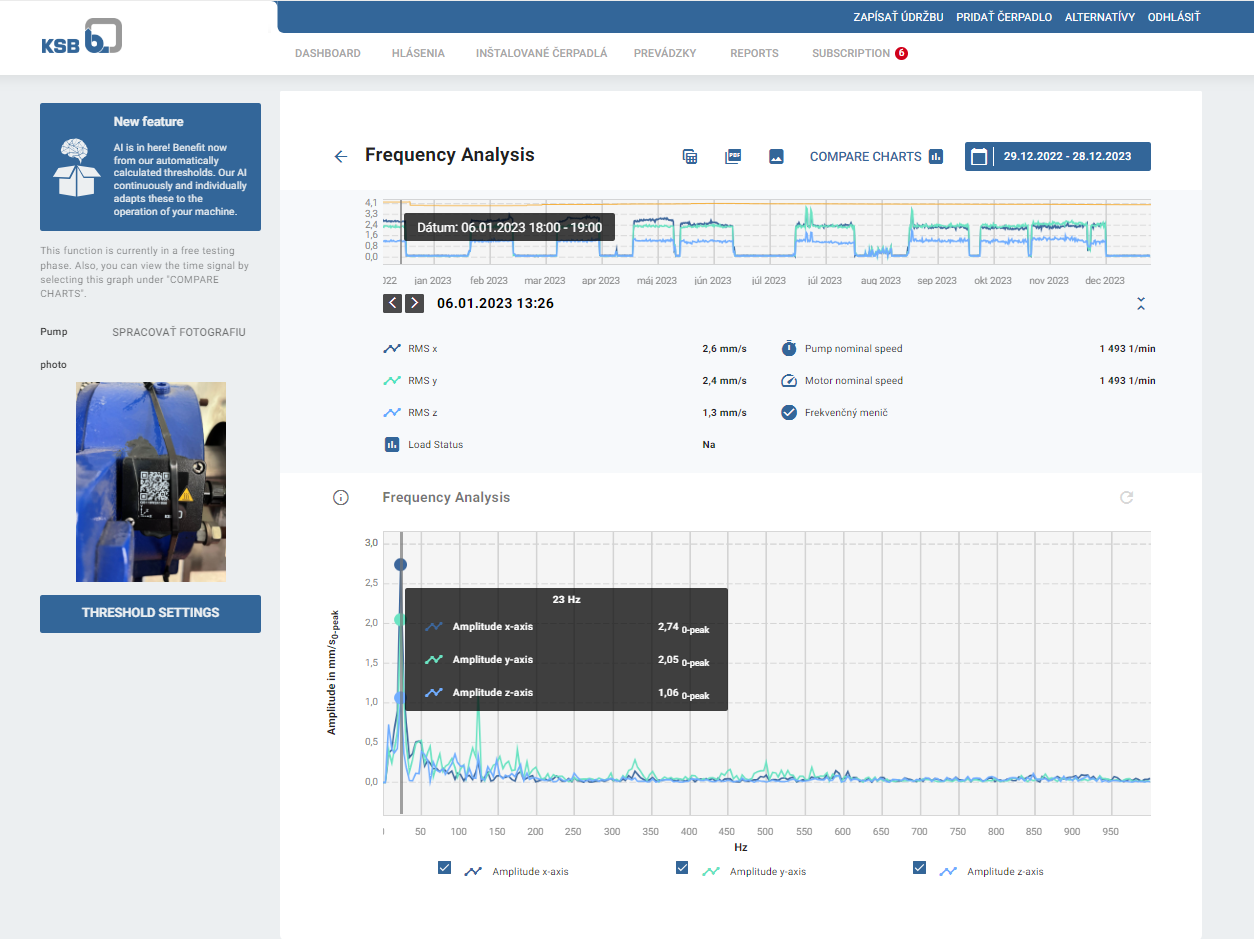
\includegraphics[width=\textwidth]{assets/design/ksb-guard-spectrum.png}
        \caption{Vibration spectral analysis dashboard}
    \end{subfigure}
     \caption{KSB Guard cloud monitoring for pumps}
     \label{fig:design:ksb-guard}
\end{figure}

\textbf{Complete schedule} for planned vibration data gathering on the designated machines and measurement procedure is described in Appendix~\ref{appendix:technical-docs}. In addition, we are able to export the entire historical record at hourly intervals. Logs from \textbf{KSB Guard} cloud monitoring tool contain vibration rms velocities and frequency spectra for two monitored KSB water pumps (Figure~\ref{fig:design:ksb-guard}).


\section{Data volume savings}
The apparent advantage of feature discovery is reducing the amount of data downstream. Data compression must occur on edge devices to enable the utilization of wireless low-power wide area networks (LPWAN). The protocol stack may differ, so goodput is compared without node configuration metadata and keepalive messages. 

The machinery monitoring system relies on determining several parameters:
\begin{itemize}
\itemsep0pt
\item \textbf{Number of source channels} ($S$): comprises the number of monitored machines, measurement locations for sensors, and active sensor axes.
\item \textbf{Sampling frequency} ($f_s$): is set based on the linear response of the accelerometer, the types of faults intended for detection, and how soon they should be noticed after they arise. The higher required sensitivity means a higher sampling rate derived according to the Nyquist theorem. At a minimum, it should be 15 kHz to 20 kHz.
\item \textbf{Interval between successive measurements} ($T$): specifies the minimal response time to sudden failure. The more critical the machine is, the interval should be shorter. The bigger the machine parts, the slower the defect evolves.
\item \textbf{Duration of valid recording} ($D$): is the captured snapshot of machine unaltered behavior associated with a timestamp. Duration should cover at least 3 windows for spectral estimation. The spectral resolution of 1 Hz amounts to 3 seconds of signal under such assumptions.
\item \textbf{Number of extracted features} ($F$): are ideally key trend indicators pointing to symptoms of common malfunctions. We aim for a total of 6 features.
\end{itemize}

Equation \ref{equ:compression-ratio-features} expresses the lossy compression ratio ($\mathcal{C}$) formula if trend indicators are stored instead of full recording. The number of raw channels ($S_{\mathrm{in}}$) can differ from those extracted in features ($S_{\mathrm{out}}$). Parameter $D = 0.5$ when we use frequency bins with 1 Hz resolution.

\myequations{Lossy compression ratio with features}
\begin{ceqn}\begin{align} \label{equ:compression-ratio-features}
\mathcal{C} = \frac{D \cdot f_s \cdot S_{\mathrm{in}}}{F \cdot S_{\mathrm{out}}}
\end{align}\end{ceqn}

\textbf{Compression ratio} for MaFaulDa dataset compared to all 21 extracted features in 3 dimensions is 2381:1. If 6 features are kept, the compression is 25000:1, which is a saving of the original data by 99.996\%.

As an example to approximate required network goodput and storage in practice, we consider continuous vibration \textbf{monitoring for municipal water pumping station}. The station has 3 pumps and 3 electric motors. 

A pump and motor pair have 4 bearings together for drive end and non-drive end positions. Each position has a sensor mounted in 3 directions that makes a total of \emph{36 source channels}. The sampling frequency at each position is set to \emph{20 kHz}. The recordings have \emph{duration of 5 seconds} and are triggered regularly every 1 hour (\emph{8760 times per year}).

In a year, the system gathers 31.54 Gs (gigasamples) which is 58.74 GiB with a 16-bit ADC resolution. Reasonably precise spectral estimation with 10 thousand bins needs 3.15 Gs per year. On the other hand, 6 features out of each channel keep only 1.89 Ms per year for a lossy compression ratio of 16667:1. Low data volumes potentially enable feature selection and models to be offloaded directly to edge devices. The entire machine's history can be kept in a small flash memory module.


\section{Data collection methodology}
% UML of experiment

% Measurement plan (calendar and folders) - dataset schema



